\chapter{Beyond Gaussianity: Laplace Innovations}\label{ch:laplace}

Every result of Chapter~\ref{ch:gaussian} rests on one algebraic miracle:
Gaussians are closed under the two operations the model performs ---
multiplying densities and marginalising. This chapter removes the miracle in
the most controlled way available: we keep the AR(1) chain, the OU channel,
and the entire factor-graph structure, and change \emph{only} the innovation
law from Gaussian to Laplace. Heavy-tailed, kinked at the origin, yet still
log-concave and analytically friendly, the Laplace distribution is the
minimal step outside the Gaussian world --- ``Laplace and Gaussian, it's not
super different'' was the supervision verdict, which is precisely why the
comparison is informative: every deviation we find is attributable to
non-Gaussianity alone, not to a change of structure. We proceed in the order
of the research programme agreed in supervision: first the $K = 1$ building
block, where the score first becomes nonlinear; then the chain $K \geq 2$,
where we exhibit the Markov-structured form of the score, a clean closed
form for the boundary message, and the precise point where closed forms die.

\section{The $K = 1$ warm-up: one frame, no chain}\label{sec:l-K1}

For $K = 1$ there is no Markov structure; the model isolates the single
ingredient ``non-Gaussian prior meets Gaussian channel''. Let
\begin{equation}
  a \sim \mathrm{Laplace}(0, b), \qquad
  p_0(a) = \frac{1}{2b}\, e^{-|a|/b}, \qquad
  \operatorname{Var}(a) = 2b^2 ,
  \label{eq:l-prior}
\end{equation}
and corrupt through the OU channel: $x = \mu a + \sqrt{\Deltat}\,\xi$ with
$\mu := e^{-t}$, $\xi \sim \Nd(0,1)$. The noised marginal is the
convolution
\begin{equation}
  p_t^{(1)}(x) = \int p_0(a)\, \Nd\big(x;\, \mu a,\, \Deltat\big)\, \dd a .
  \label{eq:l-pt1}
\end{equation}
Its limits are immediate: as $t \to 0$ the Gaussian kernel becomes a Dirac
mass and $p_t^{(1)} \to p_0$ (the kinked Laplace shape); as $t \to \infty$
the kernel loses its $a$-dependence and $p_t^{(1)} \to \Nd(0, 1)$, the OU
attractor. The family interpolates monotonically between the two
(Figure~\ref{fig:l-density}).

\begin{figure}[t]\centering
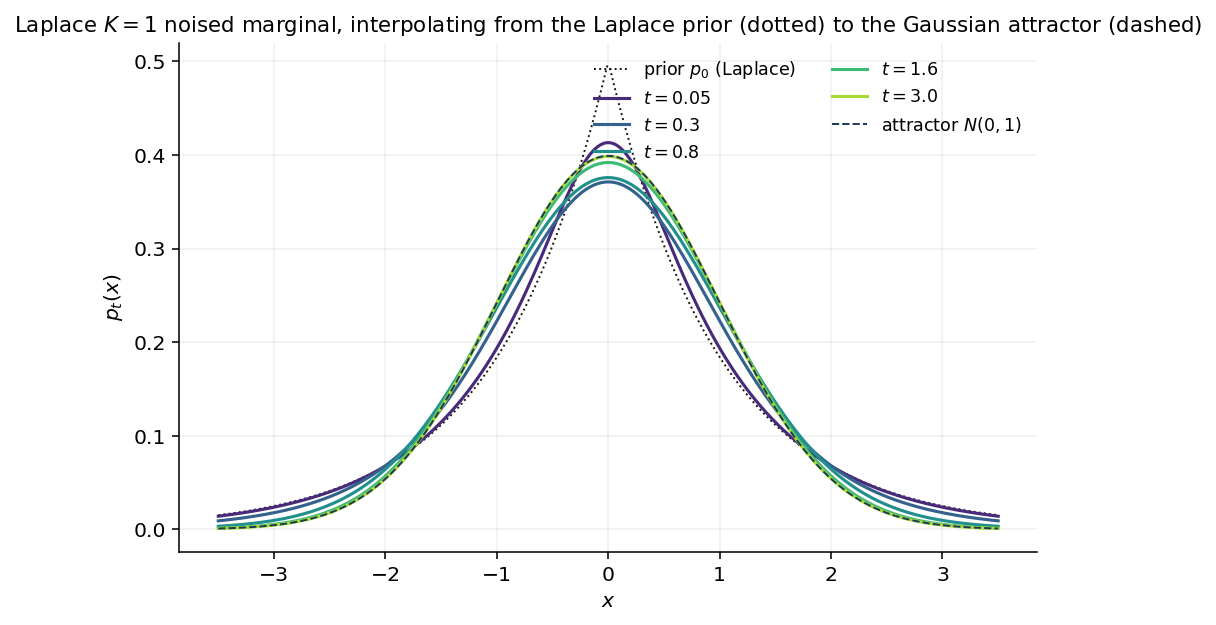
\includegraphics[width=0.8\linewidth]{figures/fig06_K1_density.png}
\caption{\textbf{Laplace $K=1$ noised marginal} ($b = 1$) at increasing
diffusion times, from the kinked Laplace prior (dotted) to the Gaussian
attractor (dashed).}
\label{fig:l-density}
\end{figure}

\subsection{The score becomes nonlinear}

Tweedie's identity \eqref{eq:tweedie} holds for \emph{any} prior:
$S(x, t) = (\mu\, \E[a|x] - x)/\Deltat$. For a Gaussian prior the
conditional mean is affine in $x$ and the score is affine; for the Laplace
prior $\E[a|x]$ interpolates nonlinearly between the regimes, and the score
inherits the nonlinearity. Its two limits are again exact
(Figure~\ref{fig:l-score-limits}):
\begin{equation}
  t \to 0:\;\; \Deltat\, S(x, t) \to -\operatorname{sign}(x)\, \cdot\, b^{-1}\!\cdot\Deltat/\Deltat
  \;\;\text{i.e.}\;\; S \sim -\frac{\operatorname{sign}(x)}{b} \cdot \frac{1}{1},
  \qquad
  t \to \infty:\;\; S(x, t) \to -x ,
  \label{eq:l-score-limits}
\end{equation}
that is: at small $t$ the score converges (after the appropriate rescaling)
to the \emph{sign-shaped} score of the Laplace prior itself,
$\partial_x \log p_0 = -\operatorname{sign}(x)/b$, with all the
nonlinearity concentrated in the kink near $x = 0$; at large $t$ it
flattens into the linear Gaussian-attractor score $-x$. The audit verifies
the Tweedie route against central finite differences of $\log p_t^{(1)}$
computed by quadrature: maximum disagreement $1.19 \times 10^{-7}$ over a
grid of $(b, t, x)$, at the truncation floor of the finite difference; the
Gaussian-attractor limit at $t = 6$ holds to $7.4 \times 10^{-6}$.

\begin{figure}[t]\centering
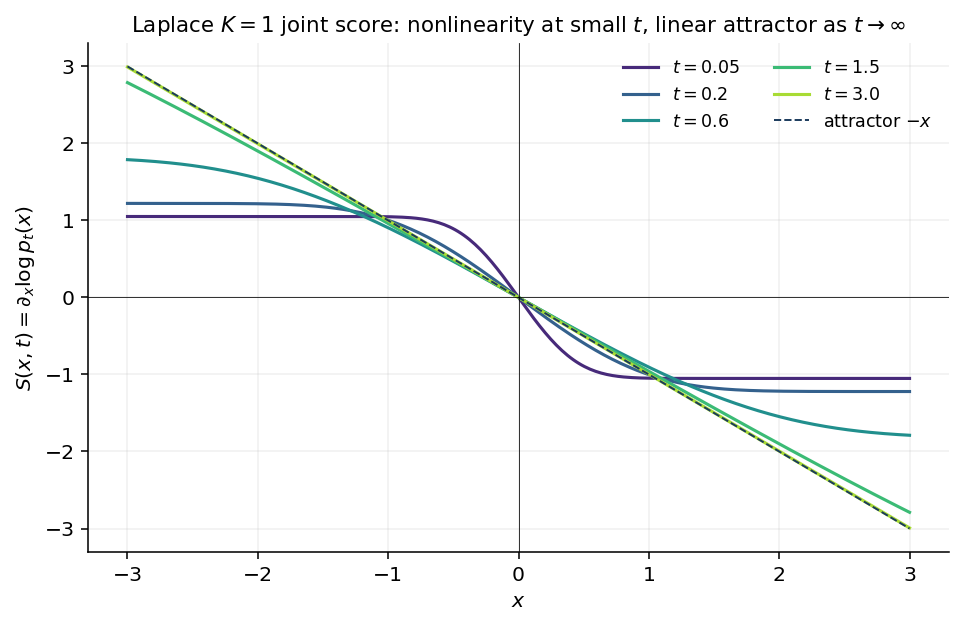
\includegraphics[width=0.8\linewidth]{figures/fig07_K1_score.png}
\caption{\textbf{Laplace $K=1$ score} at the same diffusion times as
Figure~\ref{fig:l-density}; the dashed line is the Gaussian attractor
$-x$. The nonlinearity lives in the kink near $x = 0$ and flattens as
$t$ grows.}
\label{fig:l-score}
\end{figure}

\begin{figure}[t]\centering
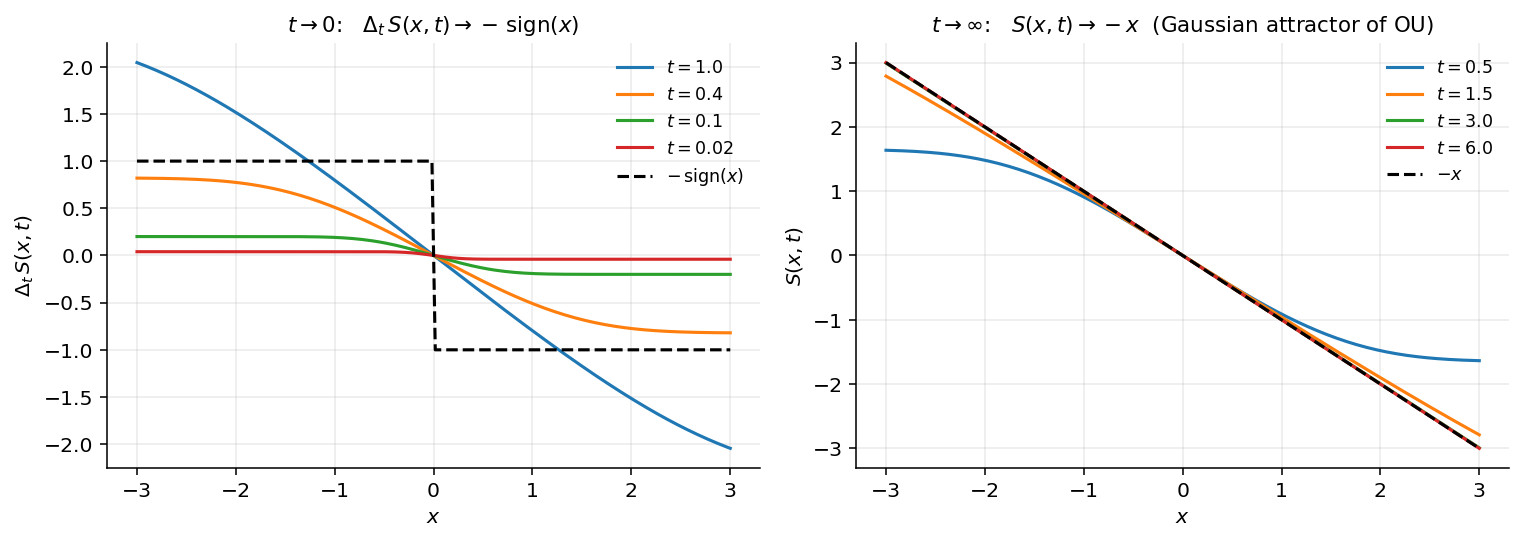
\includegraphics[width=\linewidth]{figures/fig08_K1_score_limits.png}
\caption{\textbf{Limits of the Laplace $K=1$ score} ($b=1$). Left: rescaled
score for decreasing $t$, converging pointwise to $-\operatorname{sign}(x)$.
Right: unscaled score for increasing $t$, converging to $-x$.}
\label{fig:l-score-limits}
\end{figure}

\subsection{The Fourier representation: convolution becomes product}
\label{sec:l-fourier}

The channel writes $x$ as a sum of \emph{independent} variables
($\mu a$ and $\sqrt{\Deltat}\xi$), so the density \eqref{eq:l-pt1} is a
convolution --- awkward in real space, trivial in Fourier space.

\begin{proposition}[Characteristic-function factorisation]\label{prop:l-cf}
\begin{equation}
  \widehat{p}_t^{\,(1)}(k)
  = \underbrace{\frac{1}{1 + b^2 \mu^2 k^2}}_{\text{c.f.\ of } \mu a}
    \cdot
    \underbrace{e^{-\Deltat k^2/2}}_{\text{c.f.\ of } \sqrt{\Deltat}\,\xi} .
  \label{eq:l-cf}
\end{equation}
\end{proposition}

The proof is the convolution theorem plus two standard transforms: the
Laplace characteristic function $(1 + b^2 k^2)^{-1}$ (a direct integral),
rescaled by $\mu$, and the Gaussian one. What the factorisation buys is a
\emph{differential} characterisation of the noised marginal:

\begin{theorem}[Screened Poisson equation]\label{thm:l-screened}
The Laplace noised marginal solves the linear, constant-coefficient ODE
\begin{equation}
  \boxed{\;
  \big( 1 - b^2 \mu^2\, \partial_x^2 \big)\, p_t^{(1)}(x)
  \;=\; G_{\Deltat}(x)
  \;}
  \qquad
  G_{\Deltat}(x) = \frac{e^{-x^2/2\Deltat}}{\sqrt{2\pi \Deltat}} .
  \label{eq:l-screened}
\end{equation}
\end{theorem}

\begin{toolbox}{From the characteristic function to the screened Poisson
equation}
Multiply \eqref{eq:l-cf} by $(1 + b^2\mu^2 k^2)$ to clear the rational
factor:
\begin{equation*}
  \big( 1 + b^2 \mu^2 k^2 \big)\, \widehat{p}_t^{\,(1)}(k)
  = e^{-\Deltat k^2 / 2},
\end{equation*}
whose right-hand side is exactly the characteristic function of
$G_{\Deltat}$. Now translate back to real space with the differentiation
rule: $\widehat{\partial_x f}(k) = ik\,\widehat f(k)$, applied twice, gives
$\widehat{\partial_x^2 f}(k) = -k^2 \widehat f(k)$ --- multiplication by
$k^2$ in Fourier is $-\partial_x^2$ in real space, and this single minus
sign converts $(1 + b^2\mu^2 k^2)$ into the operator
$(1 - b^2\mu^2 \partial_x^2)$. Equation \eqref{eq:l-screened} follows by
inverse-transforming term by term. The audit checks \eqref{eq:l-cf} against
direct quadrature of $\int p_t^{(1)}(x) e^{ikx} \dd x$ to
$2.9 \times 10^{-6}$, the floor of oscillatory quadrature.
\hfill$\square$
\end{toolbox}

Equation \eqref{eq:l-screened} is the structural heart of the Laplace case:
the noised marginal is the solution of a screened Poisson equation with a
Gaussian source, with screening length $b\mu = b e^{-t}$ --- the memory of
the prior's tails, shrinking with diffusion time. It also quantifies the
supervision remark that Laplace ``is not super different'' from Gaussian:
the deviation from Gaussianity is governed by a single local differential
operator whose strength dies as $e^{-t}$.

\subsection{The curvature becomes a field}

Differentiating Tweedie's identity once more,
\begin{equation}
  H_t(x) := -\partial_x^2 \log p_t^{(1)}(x)
  = \frac{1}{\Deltat}
    \left( 1 - \frac{\mu^2}{\Deltat}\, \operatorname{Var}[a \,|\, x] \right).
  \label{eq:l-curvature}
\end{equation}
For a Gaussian prior the posterior variance is $x$-independent, so $H_t$ is
a constant --- the score is affine, its Hessian flat. For the Laplace prior
$\operatorname{Var}[a|x]$ depends on $x$, and $H_t(x)$ becomes a nontrivial
\emph{field}: the breakdown of Hessian constancy is the second-order shadow
of the breakdown of score linearity, and both flow from the same source ---
a non-Gaussian prior makes $\E[a|x]$ nonlinear. This observation matters
for Chapter~\ref{ch:bp}: a Gaussian message is exactly the object that
cannot represent an $x$-dependent curvature, so \eqref{eq:l-curvature}
already tells us \emph{what} the Gaussian closure will get wrong, before we
measure \emph{how much}.

\section{The Laplace chain, $K \geq 2$}\label{sec:l-chain}

The Laplace AR(1) chain replaces the Gaussian innovations of
\eqref{eq:g-ar1} with Laplace ones:
\begin{equation}
  P_0(a) = \frac{1}{(2b)^K}
  \exp\!\left( -\frac{1}{b} \sum_{k=0}^{K-1}
    \big| a_k - \alpha a_{k-1} \big| \right),
  \qquad a_{-1} := 0 .
  \label{eq:l-chain-prior}
\end{equation}
The likelihood still factorises across frames, so the posterior inherits
the \emph{same} tree-shaped factor graph as the Gaussian model
(Proposition~\ref{prop:chain-tree}): belief propagation remains exact in
principle. What is lost is representability --- the messages are no longer
Gaussian, and computing them requires quadrature or an analytic
representation. Three structural results, corresponding to the three
threads of the supervision programme, delimit exactly what survives.

\subsection{The Markov-structured form of the joint score}

\begin{theorem}[Joint score from chain messages]\label{thm:l-markov-score}
For \emph{any} chain prior --- in particular \eqref{eq:l-chain-prior} ---
and the OU likelihood, the joint score is, componentwise,
\begin{equation}
  S_k(x, t) = \frac{\mu\, \E[a_k | x] - x_k}{\Deltat},
  \qquad
  \E[a_k | x]
  = \frac{\displaystyle\int a_k\; m_k(a_k)\; \Nd(x_k; \mu a_k, \Deltat)\;
      b_k(a_k)\;\dd a_k}
     {\displaystyle\int m_k(a_k)\; \Nd(x_k; \mu a_k, \Deltat)\;
      b_k(a_k)\;\dd a_k},
  \label{eq:l-markov-score}
\end{equation}
where $m_k$ and $b_k$ are the forward and backward BP messages into frame
$k$ (Chapter~\ref{ch:bp}).
\end{theorem}

The content of \eqref{eq:l-markov-score} --- the direct answer to
``express the score using the Markov structure'' --- is a complexity
statement: the $K$-dimensional posterior integral has been replaced by two
\emph{one-dimensional} message recursions plus one one-dimensional integral
per frame. Computational locality survives non-Gaussianity intact; what
does not survive is the collapse of those 1D integrals into closed-form
arithmetic, as we now make precise.

\subsection{The boundary message in closed form, and where closed forms
die}

\begin{proposition}[One-step Laplace integral]\label{prop:l-onestep}
For the Laplace transition $M(a'|a) = \frac{1}{2b} e^{-|a' - \alpha a|/b}$
and OU evidence $\Nd(x'; \mu a', \Deltat)$,
\begin{equation}
  \int_\R M(a' | a)\; \Nd(x'; \mu a', \Deltat)\; \dd a'
  \;=\; p_t^{(1)}\big( x' - \mu\alpha\, a \big) :
  \label{eq:l-onestep}
\end{equation}
the first backward message of the chain is the universal $K = 1$ noised
marginal, evaluated at a shifted argument.
\end{proposition}

\begin{toolbox}{Innovation change of variable, one step}
Fix $a$ and substitute the innovation $r := a' - \alpha a$; the transition
density becomes the bare Laplace prior at $r$, and the Gaussian evidence at
$a' = \alpha a + r$ becomes $\Nd(x' - \mu\alpha a;\, \mu r,\, \Deltat)$.
Hence
\begin{equation*}
  \int \frac{e^{-|r|/b}}{2b}\,
  \Nd\big( x' - \mu\alpha a;\; \mu r,\; \Deltat \big)\, \dd r
  \;=\; p_t^{(1)}\big( x' - \mu\alpha a \big)
\end{equation*}
by the very definition \eqref{eq:l-pt1}. The shift $\mu\alpha a$ is what
frame $a$ predicts for the next frame's noisy observation under the AR(1)
dynamics; the Act-one analysis of $p_t^{(1)}$ (screened Poisson equation
included) recycles wholesale as the chain's boundary building block.
\hfill$\square$
\end{toolbox}

\begin{remark}[Why iteration destroys the closed form]\label{rmk:l-breakdown}
Equation \eqref{eq:l-onestep} works because the integrand contains
\emph{exactly one} Laplace kink times \emph{exactly one} Gaussian. Every
subsequent BP step, in either direction, violates this: the incoming
message already carries the propagated structure of several frames --- a
sum of products of kinks and Gaussians --- so the next integrand contains
two or more absolute-value kinks. On each sign-quadrant the integral
reduces to half-line Gaussians, but globally it is a sum of error functions
whose arguments depend on the conditioning variable non-affinely: the clean
form does not survive one iteration. Contrast the Gaussian chain, where
every step is Gaussian-times-Gaussian and closure propagates forever. This
is the precise, structural location of the difference between the two
benchmarks --- and the precise reason the Gaussian projection of
Chapter~\ref{ch:bp} is an \emph{approximation} here, with an error to be
measured rather than an identity to be proved.
\end{remark}

\subsection{Innovation coordinates: the coupling has to live somewhere}

The one-step trick suggests decoupling the whole prior at once. Define the
triangular change of variables $r_0 = a_0$, $r_k = a_k - \alpha a_{k-1}$;
its inverse is $a = L r$ with $L_{ij} = \alpha^{i-j} \mathbf{1}_{i \geq j}$
unit lower-triangular, so the Jacobian is $1$ and
\begin{equation}
  P_0(r) = \frac{1}{(2b)^K} \prod_{k=0}^{K-1} e^{-|r_k|/b} :
  \label{eq:l-innov-prior}
\end{equation}
in innovation coordinates the prior factorises into i.i.d.\ Laplace
variables --- as decoupled as it can be. But substituting $a = Lr$ in the
likelihood produces
\begin{equation}
  p(x | r) \propto \exp\!\Big(
    -\tfrac{\mu^2}{2\Deltat}\, r^\T L^\T L\, r
    + \tfrac{\mu}{\Deltat}\, x^\T L\, r \Big),
  \label{eq:l-innov-lik}
\end{equation}
and $L^\T L$ is \emph{dense} (its entries sum geometric series in $\alpha$
and vanish nowhere). The AR(1) coupling did not disappear; it migrated from
the prior to the likelihood. In the original coordinates the prior carries
the chain and the likelihood is diagonal; in innovation coordinates the
prior is diagonal and the likelihood carries the chain. There is no basis
in which both are diagonal at once --- the non-Gaussian counterpart of the
Gaussian statement that $\Qt$ is tridiagonal in the frame basis and
diagonal in the spectral basis, but never both
(Section~\ref{sec:g-lifecycle}).

\section{What survives, what is open}

Chapter results, classified. \emph{Exact}: the noised marginal limits, the
score limits \eqref{eq:l-score-limits}, the characteristic-function
factorisation \eqref{eq:l-cf}, the screened Poisson equation
\eqref{eq:l-screened}, the Markov-structured score
\eqref{eq:l-markov-score}, the one-step boundary form
\eqref{eq:l-onestep}, the innovation factorisation
\eqref{eq:l-innov-prior}--\eqref{eq:l-innov-lik}, and the structural
breakdown argument of Remark~\ref{rmk:l-breakdown}. \emph{Numerical}: the
quadrature audits quoted above (Tweedie vs finite differences;
characteristic function vs direct integration). \emph{Open}: a
quadrature-free representation of general (non-boundary) messages at
$K \geq 2$, e.g.\ by controlled small-$\alpha$ expansion; and a
basis-independent statement of which locality of the joint score survives
non-Gaussianity (candidates: sparsity of the $x$-dependent Hessian in a
suitable basis, low-rank corrections to a tridiagonal core). An earlier
conjecture of this project --- that the Laplace $K = 2$ Hessian is
approximately rank-two --- proved regime-dependent under quick-resolution
tests and is \emph{not} asserted here.

The chapter leaves us exactly where the research programme wants us: the
Laplace chain is structurally identical to the Gaussian one (same tree,
same $O(K)$ message complexity, same Tweedie identity) but its messages are
genuinely infinite-dimensional. The question ``what does it cost to force
them Gaussian?'' is now sharply posed; Chapter~\ref{ch:bp} answers it.
